\begin{frame}{O Sistema do Telégrafo}
    \begin{itemize}
        \item \textbf{Funcionamento Eletromecânico:}
              \begin{itemize}
                  \item Circuito composto por bateria, chave (transmissor) e bobina (receptor).
                  \item O fechamento da chave cria um campo magnético que atrai uma placa metálica ("estalido").
                  \item O retorno por mola ao abrir o circuito gera um som distinto.
              \end{itemize}
        \item \textbf{Representação Digital:}
              \begin{itemize}
                  \item Uso de dois símbolos distintos: \textbf{pontos} (pulsos curtos) e \textbf{traços} (pulsos longos).
                  \item Base do Código Morse: a informação é codificada na \textbf{duração} e na \textbf{sequência} dos pulsos.
              \end{itemize}
    \end{itemize}

\end{frame}

\begin{frame}{Diagramas de Tempos e Sinais}
    \begin{center}
        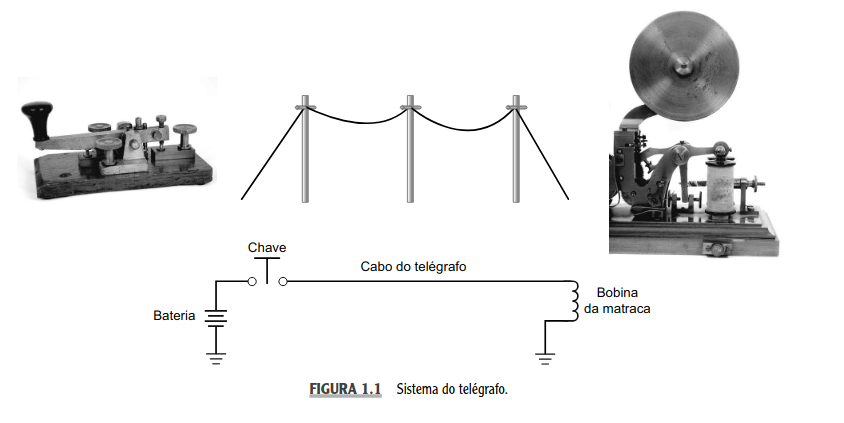
\includegraphics[width=0.8\textwidth]{Figuras/telegrafo.png}

    \end{center}
    \begin{itemize}
        \item \textbf{Natureza do Sinal:}
              \begin{itemize}
                  \item O sinal elétrico é binário: está sempre \textbf{ligado} ou \textbf{desligado}.
                  \item Precursor dos sistemas modernos (níveis lógicos 0 e 1).
              \end{itemize}
        \item \textbf{Diagrama de Tempos:}
              \begin{itemize}
                  \item Gráfico da tensão (ou corrente) versus tempo ($x = t$).
                  \item \textbf{Função:} Mostra o estado do sistema em qualquer instante e o momento exato das transições.
              \end{itemize}
    \end{itemize}





\end{frame}


\begin{frame}[t]{Diagramas de Tempo}
    \begin{itemize}
        \item Representação gráfica da atividade em sistemas digitais
        \item Eixo \textbf{x}: tempo
        \item Eixo \textbf{y}: estado (1 ou 0)
        \item Mostra:
              \begin{itemize}
                  \item Estado do sistema em qualquer momento
                  \item Momento exato das mudanças de estado
              \end{itemize}
        \item \textbf{Ferramenta fundamental} para análise de sistemas digitais
    \end{itemize}

    \begin{center}
        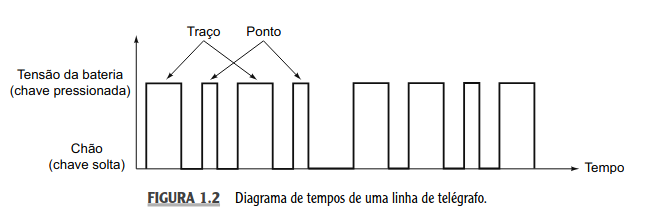
\includegraphics[width=0.9\textwidth]{Figuras/diagrama-de-tempo.png}

    \end{center}
\end{frame}

\begin{frame}{Representação Analógica}
    \begin{itemize}
        \item \textbf{Definição:} Uma quantidade é representada por um indicador proporcional \textbf{continuamente variável}.
        \item \textbf{Características Principais:}
              \begin{itemize}
                  \item Acompanha variações mínimas de forma fluida.
                  \item O indicador (ponteiro, coluna, tensão) "segue" a grandeza física.
              \end{itemize}
        \item \textbf{Exemplos Clássicos:}
              \begin{itemize}
                  \item \textbf{Velocímetro Mecânico:} Deflexão do ponteiro proporcional à velocidade do eixo.
                  \item \textbf{Termômetro de Mercúrio:} Altura da coluna varia com a temperatura.
                  \item \textbf{Termômetro de Mola:} Expansão/contração térmica converte-se em posição angular.
              \end{itemize}
    \end{itemize}
\end{frame}

\begin{frame}{Sistemas Analógicos Elétricos}
    \begin{itemize}
        \item \textbf{Conversão de Grandezas:}
              \begin{itemize}
                  \item A quantidade física original é convertida em um \textbf{sinal elétrico}.
                  \item A \textbf{tensão} ou \textbf{corrente} resultante é diretamente proporcional à medida.
              \end{itemize}
        \item \textbf{Aplicações:}
              \begin{itemize}
                  \item Exibição em escalas graduadas.
                  \item Processamento de sinais em tempo real.
                  \item Sistemas de controle contínuo.
              \end{itemize}
    \end{itemize}
    \vspace{0.3cm}

\end{frame}

\begin{frame}{O Som como Grandeza Analógica}
    \begin{itemize}
        \item \textbf{Histórico:} Alexander Graham Bell (1875) converteu voz em sinal elétrico continuamente variável.
        \item \textbf{O Microfone:} Atua como um transdutor que converte energia sonora em \textbf{tensão analógica}.
        \item \textbf{Características do Sinal de Voz:}
              \begin{itemize}
                  \item \textbf{Frequência ($f$):} Ciclos por segundo; define os tons da voz.
                  \item \textbf{Período ($T$):} Tempo de cada ciclo ($T = 1/f$).
                  \item \textbf{Amplitude:} Medida no eixo vertical (Volts); define a \textbf{intensidade} (volume) e a inflexão da fala.
              \end{itemize}
    \end{itemize}

\end{frame}

\begin{frame}{Onda de Audio}
    \begin{center}
        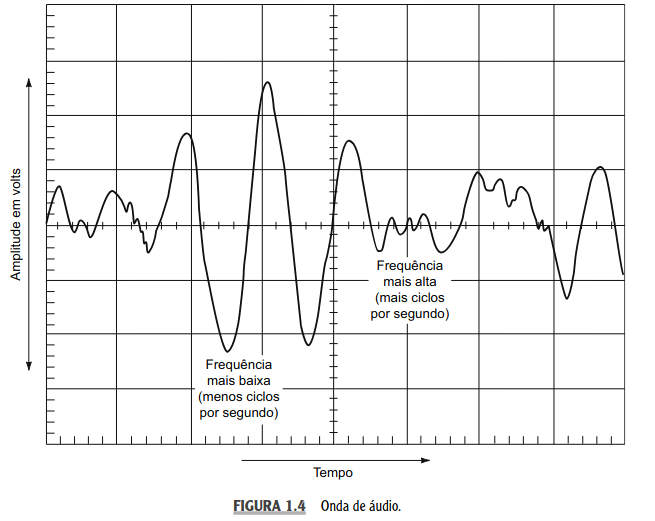
\includegraphics[width=0.7\textwidth]{Figuras/onda-de-audio.png}

    \end{center}


\end{frame}

\begin{frame}{A Natureza Contínua das Quantidades}
    \begin{itemize}
        \item \textbf{Característica Fundamental:} Variam ao longo de uma \textbf{faixa contínua} de valores.
        \item \textbf{Exemplos de Faixas Típicas:}
    \end{itemize}
    \begin{table}[]
        \centering
        \begin{tabular}{|l|l|}
            \hline
            \textbf{Grandeza}  & \textbf{Exemplo de Faixa} \\ \hline
            Velocidade         & 0 a 160 km/h              \\ \hline
            Temperatura        & -29°C a 49°C              \\ \hline
            Tensão (Microfone) & 0 a $V_{max}$             \\ \hline
        \end{tabular}
    \end{table}
    \begin{block}{Conclusão}
        Diferente do digital (degraus), o analógico não possui "saltos"; entre dois valores quaisquer, existe uma infinidade de valores intermediários.
    \end{block}
\end{frame}

\begin{frame}{Representação Digital}
    \begin{itemize}
        \item \textbf{Definição:} Quantidades representadas por símbolos chamados \textbf{dígitos}, em vez de indicadores contínuos.
        \item \textbf{Funcionamento:}
              \begin{itemize}
                  \item A variação ocorre em \textbf{incrementos discretos} (saltos).
                  \item Exemplo: Um termômetro digital que mede de $0,1^{\circ}\text{C}$ em $0,1^{\circ}\text{C}$.
                  \item A temperatura real sobe de forma fluida, mas o visor "pula" de $22,0^{\circ}\text{C}$ para $22,1^{\circ}\text{C}$.
              \end{itemize}
    \end{itemize}
    \vspace{0.3cm}
    \begin{center}
        \begin{tabular}{|c|c|}
            \hline
            \textbf{Analógica}    & \textbf{Digital}          \\ \hline
            Contínua              & Discreta (Passo a passo)  \\ \hline
            Infinidade de valores & Valores finitos/definidos \\ \hline
        \end{tabular}
    \end{center}
\end{frame}

\begin{frame}{Analógico vs. Digital}
    \begin{itemize}
        \item \textbf{Comparação Visual:}
              \begin{itemize}
                  \item O analógico é como uma \textbf{rampa} (suave).
                  \item O digital é como uma \textbf{escada} (degraus).
              \end{itemize}
        \item \textbf{Precisão e Resolução:}
              \begin{itemize}
                  \item No digital, a precisão depende do número de dígitos ou "passos" disponíveis no sistema.
              \end{itemize}
    \end{itemize}

    \begin{block}{Diferença Fundamental}
        \centering
        \textbf{Analógica $\equiv$ Contínua} \\
        \textbf{Digital $\equiv$ Discreta}
    \end{block}
\end{frame}

\begin{frame}{Ambiguidade vs. Precisão Digital}
    \begin{itemize}
        \item \textbf{Interpretação Analógica:}
              \begin{itemize}
                  \item Frequentemente sujeita a interpretação livre (ex: posição exata de um ponteiro entre dois traços).
                  \item Depende da percepção do observador.
              \end{itemize}
        \item \textbf{Ausência de Ambiguidade Digital:}
              \begin{itemize}
                  \item A leitura é direta e numérica.
                  \item Não há dúvida sobre o valor exibido (ex: $22,5^{\circ}\text{C}$ é lido exatamente como tal).
              \end{itemize}
        \item \textbf{O Processo de Digitalização:}
              \begin{itemize}
                  \item Na prática, sempre "arredondamos" medidas analógicas para um nível de precisão conveniente.
                  \item \textbf{Digitalizar:} Atribuir um número de \textbf{precisão limitada} a uma quantidade continuamente variável.
              \end{itemize}
    \end{itemize}
\end{frame}

\begin{frame}{Utilidade das Representações Digitais}
    \begin{itemize}
        \item \textbf{Captura do Mundo Real:}
              \begin{itemize}
                  \item O mundo é analógico (variáveis mudam constantemente).
                  \item Ao medir e converter essas variáveis em quantidades digitais, ganhamos novas possibilidades.
              \end{itemize}
        \item \textbf{Vantagens do Processamento Digital:}
              \begin{itemize}
                  \item \textbf{Registro:} Armazenamento fiel de dados ao longo do tempo.
                  \item \textbf{Manipulação:} Cálculos aritméticos e algoritmos complexos.
                  \item \textbf{Controle:} Uso das informações para acionar ou gerenciar sistemas.
              \end{itemize}
    \end{itemize}

\end{frame}

\begin{frame}{Quiz - Analógico ou digital?}
    \begin{center}
        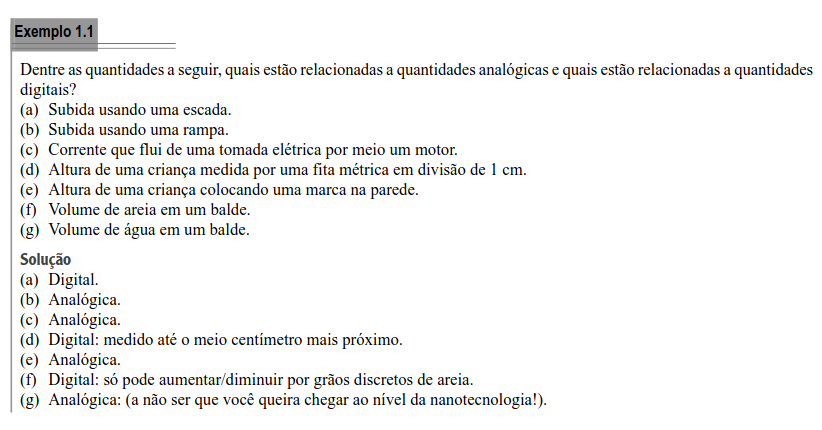
\includegraphics[width=\textwidth]{Figuras/quiz-analogico-digital.png}

    \end{center}


\end{frame}

\begin{frame}{Definição de Sistemas}
    \begin{itemize}
        \item \textbf{Sistemas Digitais:}
              \begin{itemize}
                  \item Combinação de dispositivos para manipular informação lógica ou quantidades em \textbf{valores discretos}.
                  \item \textbf{Meios:} Eletrônicos (mais comuns), mecânicos, magnéticos ou pneumáticos.
                  \item \textbf{Exemplos:} Computadores, calculadoras, sistemas de telecomunicações.
              \end{itemize}
        \item \textbf{Sistemas Analógicos:}
              \begin{itemize}
                  \item Dispositivos que manipulam quantidades em \textbf{faixas contínuas}.
                  \item \textbf{Exemplo:} O sinal de saída de um alto-falante (pode assumir qualquer amplitude entre zero e o máximo).
              \end{itemize}
    \end{itemize}
\end{frame}

\begin{frame}{Sistemas de Sinal Híbrido ou Misto}
    \begin{itemize}
        \item \textbf{Integração:} É comum o uso de ambas as técnicas em um mesmo projeto para aproveitar as vantagens específicas de cada uma.
        \item \textbf{Desafio de Projeto:} Determinar quais partes do fluxo devem ser analógicas e quais devem ser digitais.
        \item \textbf{Tendência Atual:}
              \begin{enumerate}
                  \item Digitalizar o sinal \textbf{o mais cedo possível}.
                  \item Processar digitalmente.
                  \item Converter de volta para analógico \textbf{o mais tarde possível}.
              \end{enumerate}
    \end{itemize}




    A digitalização precoce preserva a integridade da informação contra ruídos e facilita o processamento complexo.

\end{frame}

\begin{frame}{Evolução do Telefone: Um Sistema Híbrido}
    \begin{itemize}
        \item \textbf{A Visão de Bell:} Para utilidade real, os telefones precisavam funcionar em \textbf{rede}.
        \item \textbf{Sinalização (Digital):}
              \begin{itemize}
                  \item Gerador a manivela produzia tensão para as campainhas.
                  \item Cada usuário possuía um \textbf{código único} de toques (curtos e longos).
                  \item \textbf{Codificação:} Feita manualmente pelo emissor ao girar a manivela.
                  \item \textbf{Decodificação:} Feita mentalmente pelo receptor ao ouvir o padrão.
              \end{itemize}
        \item \textbf{Comunicação (Analógica):}
              \begin{itemize}
                  \item Uma vez estabelecida a conexão, a voz era transmitida de forma puramente analógica.
              \end{itemize}
    \end{itemize}
    \emph{Conceito Histórico}:
    O sistema de telefonia inicial já utilizava o conceito de \textbf{sinalização digital} para endereçamento e \textbf{transmissão analógica} para o conteúdo.

\end{frame}

\begin{frame}{Evolução: Telefones de Disco e Teclas}
    \begin{itemize}
        \item \textbf{Telefone de Disco (Pulsos):}
              \begin{itemize}
                  \item Sistema de numeração decimal representado por séries de pulsos.
                  \item \textbf{Mecanismo:} A mola de retorno girava um eixo de came que abria/fechava contatos.
                  \item \textbf{Exemplo:} 9 pulsos = número 9; 10 pulsos = número 0.
                  \item \textbf{Decodificação:} Máquinas eletromecânicas interpretavam os pulsos para realizar a conexão automática.
              \end{itemize}
        \item \textbf{Telefone de Teclas (DTMF):}
              \begin{itemize}
                  \item \textbf{DTMF:} \textit{Dual Tone Multiple Frequency}.
                  \item Cada dígito é representado por um sinal audível composto pela combinação de \textbf{duas frequências senoidais}.
                  \item Circuitos eletrônicos reconhecem os tons e os traduzem em sequência digital.
              \end{itemize}
    \end{itemize}
    \begin{block}{Integração}
        A informação digital (números) é enviada via sinais analógicos (tons), demonstrando a coexistência histórica das duas tecnologias.
    \end{block}
\end{frame}

\begin{frame}{Vantagens das Técnicas Digitais (1/2)}
    \begin{itemize}
        \item \textbf{Facilidade de Projeto:}
              \begin{itemize}
                  \item Baseado em circuitos de \textbf{chaveamento}.
                  \item Importam apenas as faixas (\textit{HIGH} ou \textit{LOW}), não valores exatos de tensão.
              \end{itemize}
        \item \textbf{Armazenamento Eficiente:}
              \begin{itemize}
                  \item Dispositivos especiais (\textit{latches}) mantêm a informação indefinidamente.
                  \item Armazenamento de massa: bilhões de bits em espaços reduzidos.
              \end{itemize}
        \item \textbf{Precisão e Exatidão:}
              \begin{itemize}
                  \item A informação não se deteriora durante o processamento.
                  \item Sistemas analógicos sofrem com variações de temperatura, umidade e tolerância de componentes.
              \end{itemize}
    \end{itemize}
\end{frame}

\begin{frame}{Vantagens das Técnicas Digitais (2/2)}
    \begin{itemize}
        \item \textbf{Operações Programáveis:}
              \begin{itemize}
                  \item Comportamento controlado por conjuntos de instruções (programas).
                  \item Flexibilidade e complexidade muito superiores aos sistemas analógicos.
              \end{itemize}
        \item \textbf{Imunidade ao Ruído:}
              \begin{itemize}
                  \item Flutuações de tensão (ruído) são desprezíveis, desde que não alterem a distinção entre nível \textbf{ALTO} e \textbf{BAIXO}.
              \end{itemize}

        \item \textbf{Alta Integração (CIs):}
              \begin{itemize}
                  \item Chips digitais comportam milhões de dispositivos.
                  \item Analógicos exigem componentes difíceis de integrar (grandes capacitores, indutores, resistores de precisão).
              \end{itemize}
    \end{itemize}
\end{frame}

\begin{frame}{Limitações das Técnicas Digitais}
    Apesar das vantagens, existem dois desafios principais na adoção do digital:
    \begin{itemize}
        \item \textbf{O Mundo Real é Analógico:}
              \begin{itemize}
                  \item Grandezas físicas (temperatura, pressão, velocidade, vazão) são contínuas por natureza.
                  \item Representações como "18°C" são apenas \textbf{aproximações digitais} da realidade.
              \end{itemize}
        \item \textbf{Tempo de Processamento:}
              \begin{itemize}
                  \item Converter, processar e desconverter sinais exige tempo (latência), o que pode ser crítico em sistemas de altíssima velocidade.
              \end{itemize}
    \end{itemize}
    \begin{exampleblock}{Exemplos de Sensores no Automóvel}
        Nível de combustível, temperatura do motor, acelerômetros (airbag) e sensores de pressão.
    \end{exampleblock}
\end{frame}

\begin{frame}{Lidando com o Mundo Analógico}
    Para integrar o processamento digital ao mundo físico, seguimos quatro passos fundamentais:
    \begin{enumerate}
        \item \textbf{Transdução:} Converter a variável física (ex: calor) em sinal elétrico analógico.
        \item \textbf{Conversão A/D:} Transformar o sinal analógico em formato digital (bits).
        \item \textbf{Processamento:} Operar a informação digitalmente (cálculos, lógica).
        \item \textbf{Conversão D/A:} Converter o resultado digital de volta para o formato analógico do mundo real.
    \end{enumerate}

\end{frame}

\begin{frame}{Estudo de Caso: Controle de Temperatura}
    \begin{itemize}
        \item \textbf{Entrada de Usuário (Digital):} Ajuste da temperatura desejada em incrementos discretos (ex: $0,1^{\circ}\text{C}$).
        \item \textbf{Captura (Analógica):} Um sensor converte a temperatura ambiente em uma \textbf{tensão proporcional}.
        \item \textbf{Interface de Processamento:}
              \begin{itemize}
                  \item \textbf{ADC (Conversor Analógico-Digital):} Traduz a tensão do sensor para um valor binário.
                  \item \textbf{Processador:} Compara o valor real com o desejado e calcula a correção necessária.
              \end{itemize}
    \end{itemize}

\end{frame}

\begin{frame}{Atuação e Ciclo de Controle}
    \begin{itemize}
        \item \textbf{Saída do Sistema:}
              \begin{itemize}
                  \item \textbf{DAC (Conversor Digital-Analógico):} Converte o ajuste digital calculado de volta para uma \textbf{tensão analógica}.
                  \item \textbf{Atuador:} O dispositivo de aquecimento recebe essa tensão e gera calor proporcional para o ambiente.
              \end{itemize}
        \item \textbf{Resumo do Fluxo:}
    \end{itemize}
    \begin{center}
        \fbox{Temp. Física} $\rightarrow$ \textbf{Sensor} $\rightarrow$ \textbf{ADC} $\rightarrow$ \textbf{Lógica Digital} $\rightarrow$ \textbf{DAC} $\rightarrow$ \textbf{Aquecedor}
    \end{center}
    \begin{block}{Importância da Conversão}
        Este ciclo permite que a precisão da lógica digital controle variáveis instáveis e contínuas do mundo físico.
    \end{block}
\end{frame}

\begin{frame}{Exemplo}
    \begin{center}
        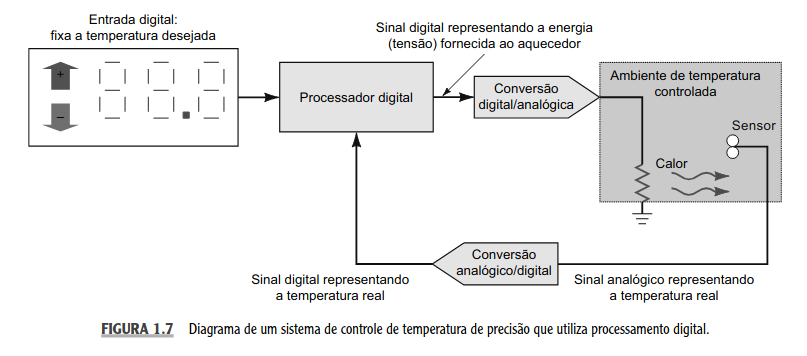
\includegraphics[width=\textwidth]{Figuras/temperatura-procdigital.png}

    \end{center}


\end{frame}

\begin{frame}{Exemplo de Transdutor: O LDR}
    \begin{itemize}
        \item \textbf{Definição:} O \textit{Light Dependent Resistor} (Resistor Dependente de Luz) é um componente analógico cuja resistência varia com a intensidade luminosa.
        \item \textbf{Comportamento Analógico:}
              \begin{itemize}
                  \item Varia a resistencia com a luz.
                  \item A variação é \textbf{contínua} e proporcional à luz recebida.
              \end{itemize}
        \item \textbf{Integração Digital:}
              \begin{itemize}
                  \item O LDR envia uma \textbf{tensão analógica} para um pino do microcontrolador.
                  \item O \textbf{ADC} interno converte essa tensão em um número.
              \end{itemize}
    \end{itemize}


\end{frame}

\begin{frame}[fragile]{Exemplo Prático: Leitura Analógica (Arduino)}
    \begin{itemize}
        \item Captura de um sinal analógico e sua conversão digital via \textbf{ADC}.
        \item A função \texttt{analogRead()} transforma a tensão no pino A0 em um valor digital.
    \end{itemize}

    \begin{exampleblock}{Código de Leitura do LDR}
        \begin{verbatim}
int ldr = A0;
int valorldr = 0;

void setup() {
  pinMode(ldr, INPUT);
  Serial.begin(9600);
}
void loop() {
   valorldr = analogRead(ldr);
   Serial.print("Valor lido pelo LDR = ");
   Serial.println(valorldr);
}
\end{verbatim}
    \end{exampleblock}
\end{frame}

\begin{frame}{Leitor de Luminosidade}
    \begin{columns}
        \begin{column}{0.5\textwidth}
            \begin{figure}
                \centering
                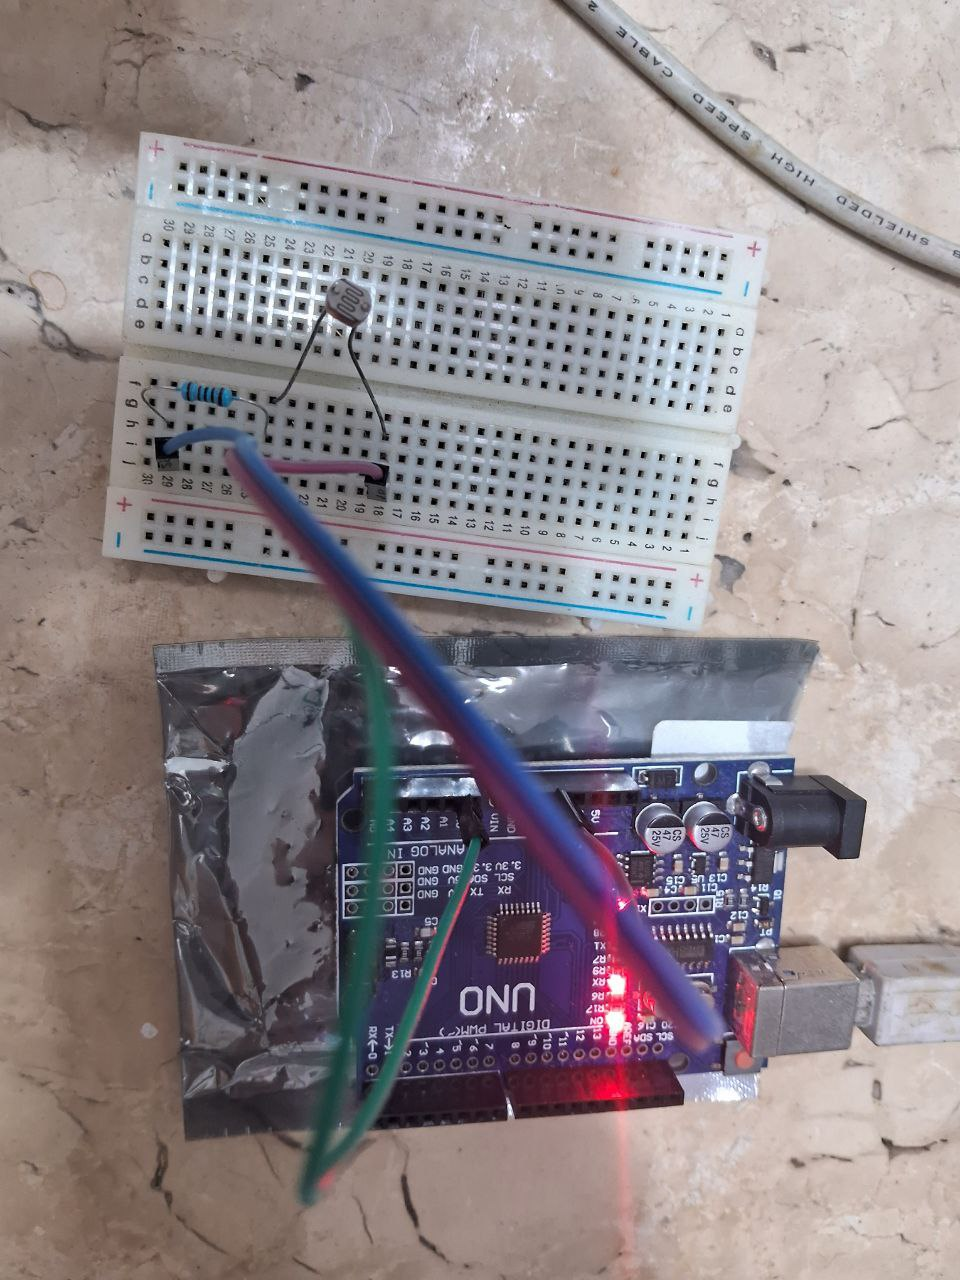
\includegraphics[width=\textwidth]{Figuras/ldr1.jpg}

            \end{figure}
        \end{column}

        \begin{column}{0.5\textwidth}
            \begin{figure}
                \centering
                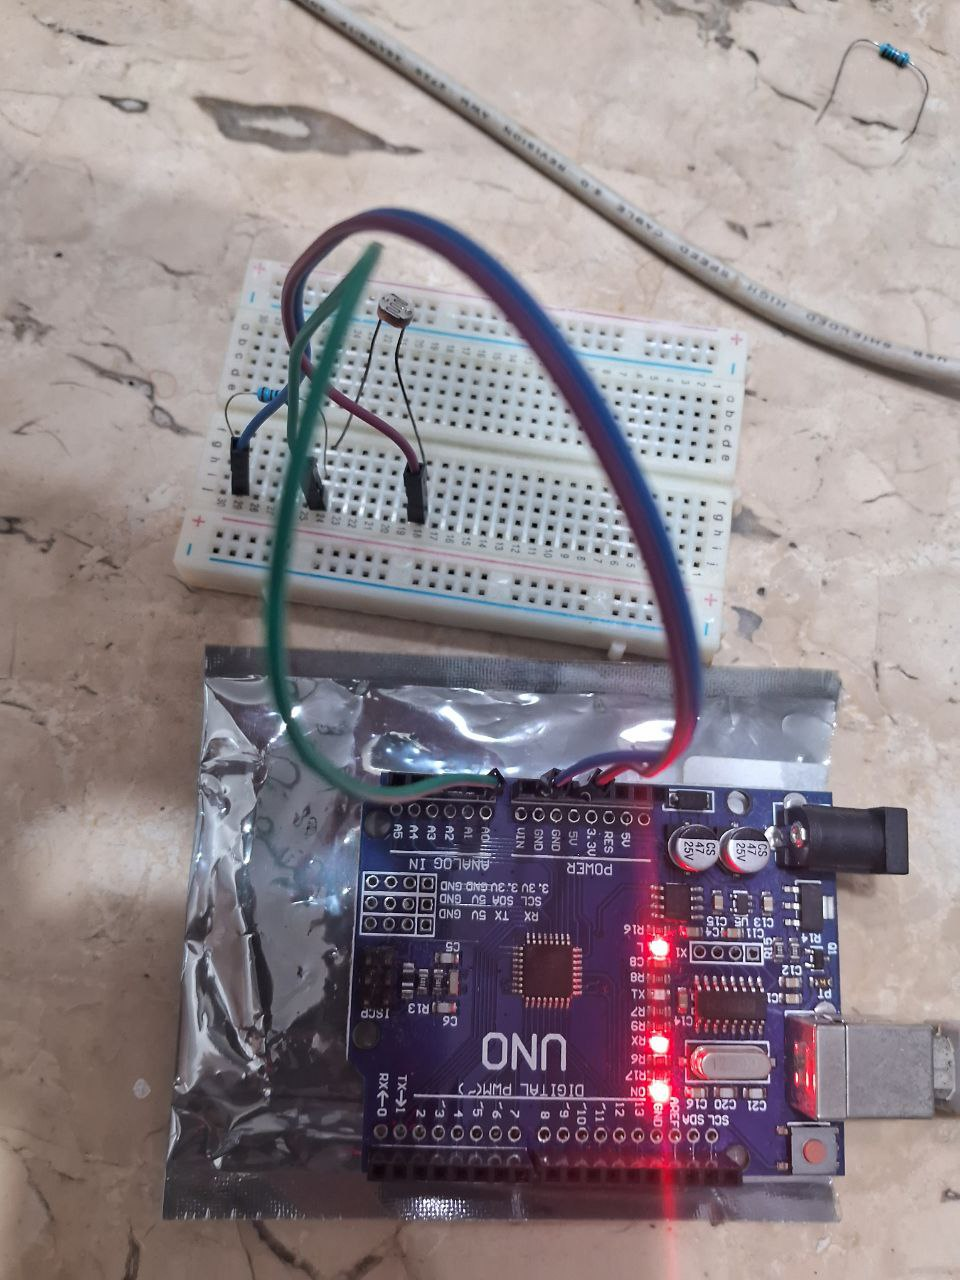
\includegraphics[width=\textwidth]{Figuras/ldr2.jpg}

            \end{figure}
        \end{column}
    \end{columns}
\end{frame}

\begin{frame}{Função \texttt{analogRead()}}
    \begin{itemize}
        \item \textbf{Descrição:} Lê o valor de um pino de entrada analógica especificado.
        \item \textbf{Conversor Analógico-Digital (ADC):}
              \begin{itemize}
                  \item O Arduino UNO possui um ADC de \textbf{10 bits}.
                  \item Mapeia tensões entre $0$ e $5\,\text{V}$ em valores inteiros entre \textbf{0 e 1023}.
              \end{itemize}
        \item \textbf{Resolução do Sistema:}
              \begin{itemize}
                  \item Cálculo: $\frac{5\,\text{V}}{1024 \text{ unidades}} \approx 0,0049\,\text{V}$ ($4,9\,\text{mV}$) por unidade.
              \end{itemize}
    \end{itemize}



    \begin{block}{Observações Técnicas}
        \begin{itemize}
            \item \textbf{analogReference():} Altera a faixa de tensão de entrada.
            \item \textbf{analogReadResolution():} Permite alterar a resolução em placas que suportam mais de 10 bits.
        \end{itemize}
    \end{block}

    \href{https://docs.arduino.cc/language-reference/en/functions/analog-io/analogRead/}{Link da API de referência}
\end{frame}

\begin{frame}{Lógica de Medição Indireta}
    \begin{itemize}
        \item \textbf{Uma cadeia:}
              \begin{enumerate}
                  \item \textbf{Fenômeno Físico:} Intensidade de luz varia.
                  \item \textbf{Efeito Analógico:} A resistência do LDR muda, alterando a \textbf{tensão ($V$)} no divisor de tensão.
                  \item \textbf{Processamento:} O microcontrolador lê essa tensão contínua.
                  \item \textbf{Interpretação:} O software associa o valor digital à condição de "escuro".
              \end{enumerate}
    \end{itemize}



    \vspace{0.3cm}
    \centering
    Nesse caso medimos a luz indiretamente através da tradução de grandezas elétricas
\end{frame}

\begin{frame}{Sistemas de Numeração Digital}
    \begin{itemize}
        \item \textbf{Panorama Geral:} Na tecnologia digital, utilizamos diferentes bases numéricas para finalidades específicas.
        \item \textbf{Os Três Pilares:}
              \begin{itemize}
                  \item \textbf{Decimal (Base 10):} Sistema utilizado por humanos no dia a dia.
                  \item \textbf{Binário (Base 2):} Linguagem nativa dos sistemas digitais (níveis lógicos).
                  \item \textbf{Hexadecimal (Base 16):} Forma compacta que facilita para humanos a leitura e escrita de grandes sequências binárias.
              \end{itemize}
    \end{itemize}



    \begin{block}{Princípio Unificado}
        Embora as bases sejam diferentes, todos esses sistemas funcionam sob a mesma lógica posicional. Entender a fundo o sistema decimal é a chave para dominar os demais.
    \end{block}
\end{frame}

\begin{frame}{Sistema Decimal (Base 10)}
    \begin{itemize}
        \item \textbf{Símbolos:} Composto por 10 dígitos: $\{0, 1, 2, 3, 4, 5, 6, 7, 8, 9\}$.
        \item \textbf{Origem:} Evoluiu do uso dos dez dedos das mãos para contagem
        \item \textit{dígito} vem do latim \textit{digitus}, "dedo".
        \item \textbf{Sistema Posicional:} O valor de um dígito depende da sua posição no número.
    \end{itemize}

    \begin{exampleblock}{Exemplo: Número 453}
        \centering
        \begin{tabular}{c c c}
            \textbf{4}        & \textbf{5}       & \textbf{3}        \\
            Centenas ($10^2$) & Dezenas ($10^1$) & Unidades ($10^0$) \\
        \end{tabular}
    \end{exampleblock}

    \begin{itemize}
        \item \textbf{MSD (Most Significant Digit):} O dígito de maior peso (neste caso, o \textbf{4}).
        \item \textbf{LSD (Least Significant Digit):} O dígito de menor peso (neste caso, o \textbf{3}).
    \end{itemize}

\end{frame}

\begin{frame}{Valor Posicional e Potências de 10}
    \begin{itemize}
        \item \textbf{A Vírgula Decimal:} Atua como o separador entre a parte \textbf{inteira} (potências positivas) e a parte \textbf{fracionária} (potências negativas).
        \item \textbf{Estrutura de Pesos:} Cada posição possui um peso que é uma potência de 10 ($10^n$).
    \end{itemize}

    \begin{exampleblock}{Decomposição do número 2745,214}
        $$ (2 \times 10^3) + (7 \times 10^2) + (4 \times 10^1) + (5 \times 10^0) + (2 \times 10^{-1}) + (1 \times 10^{-2}) + (4 \times 10^{-3}) $$
    \end{exampleblock}

    \begin{itemize}
        \item \textbf{Regra Geral:} Qualquer número é a soma dos produtos de cada dígito pelo seu valor posicional.
    \end{itemize}


\end{frame}

\begin{frame}{Exemplo}
    \begin{center}
        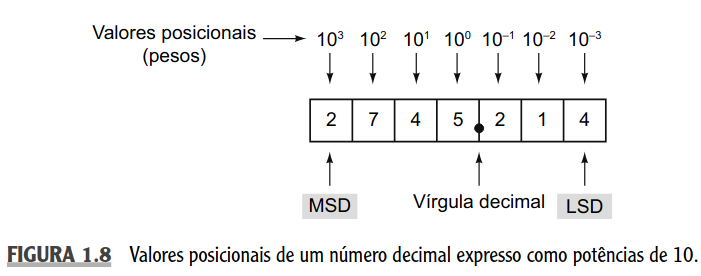
\includegraphics[width=\textwidth]{Figuras/MSDLSD.png}

    \end{center}


\end{frame}